\documentclass[t]{beamer}
\usepackage[T1]{fontenc}
\usepackage[utf8]{inputenc}  % to be able to type unicode text directly
%\usepackage[french]{babel}   % french typographical conventions
\usepackage{inconsolata}     % for a nicer (e.g. non-courier) tt family font
%\usepackage{amsthm,amsmath}  % fancier mathematics
%\usepackage{array} % to fine-tune tabular spacing
\usepackage{bbm} % for blackboard 1

\usepackage{graphicx}        % to include images
%\usepackage{animate}         % to include animated images
\usepackage{soul}            % for colored strikethrough
%\usepackage{bbding}          % for Checkmark and XSolidBrush
\usepackage{hyperref,url}

\colorlet{darkgreen}{black!50!green}  % used for page numbers
\definecolor{term}{rgb}{.9,.9,.9}     % used for code insets

\setlength{\parindent}{0em}
\setlength{\parskip}{1em}


% coco's macros
\def\R{\mathbf{R}}
\def\F{\mathcal{F}}
\def\x{\mathbf{x}}
\def\y{\mathbf{y}}
\def\u{\mathbf{u}}
\def\Z{\mathbf{Z}}
\def\ud{\mathrm{d}}
\DeclareMathOperator*{\argmin}{arg\,min}
\DeclareMathOperator*{\argmax}{arg\,max}
\newcommand{\reference}[1] {{\scriptsize \color{gray}  #1 }}
\newcommand{\referencep}[1] {{\tiny \color{gray}  #1 }}
\newcommand{\unit}[1] {{\tiny \color{gray}  #1 }}

% disable spacing around verbatim
\usepackage{etoolbox}
\makeatletter\preto{\@verbatim}{\topsep=0pt \partopsep=0pt }\makeatother

% disable headings, set slide numbers in green
\mode<all>\setbeamertemplate{navigation symbols}{}
\defbeamertemplate*{footline}{pagecount}{\leavevmode\hfill\color{darkgreen}
   \insertframenumber{} / \inserttotalframenumber\hspace*{2ex}\vskip0pt}

%% select red color for strikethrough
\makeatletter
\newcommand\SoulColor{%
  \let\set@color\beamerorig@set@color
  \let\reset@color\beamerorig@reset@color}
\makeatother
\newcommand<>{\St}[1]{\only#2{\SoulColor\st{#1}}}
\setstcolor{red}

% make everything monospace
\renewcommand*\familydefault{\ttdefault}

% define a font size tinier than tiny
\makeatletter
\newcommand{\srcsize}{\@setfontsize{\srcsize}{5pt}{5pt}}
\makeatother


\begin{document}

\addtocounter{framenumber}{-1}
\begin{frame}[plain,fragile]
\LARGE\begin{verbatim}





     The Kernel Rank Transform




rafa & enric
gtti 21-11-2024
\end{verbatim}
\end{frame}


\begin{frame}
THE KERNEL RANK TRANSFORM IN ONE SLIDE\\
======================================

{\bf Definition:}
{\color{blue}
	\fbox{
		\color{black}
		\(\displaystyle
		\textsc{KRT}_{{\color{red}\kappa},{\color{red}\sigma}}({\color{blue}u})({\color{blue}x})
		:=
		\int {\color{red}\kappa}({\color{blue}x}-y)\,{\color{red}\sigma}({\color{blue}u(x)}-{\color{blue}u}(y))\,\ud y
		\)
	}
}

\vspace{-0.5em}

{\bf Examples:}

\vspace{-1em}

%MAKE all: o/introex5.png o/introex30.png o/introex99.png o/introex190.png
%MAKE o/introex%.png:  i/barbsquare.png; ./krt actualsquare$* $^|qauto -i - $@
\begin{tabular}{cccc}
	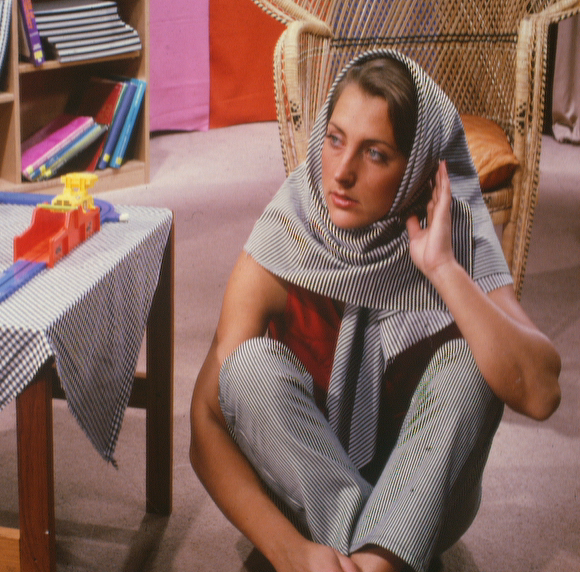
\includegraphics[width=0.2\linewidth]{i/barbara.png}&
	\includegraphics[width=0.2\linewidth]{o/introex5.png}&
	\includegraphics[width=0.2\linewidth]{o/introex30.png}&
	\includegraphics[width=0.2\linewidth]{o/introex190.png}\\
	$u$ &
	$\footnotesize\textsc{KRT}_{{\color{red}g_5},H}(u)$ &
	$\footnotesize\textsc{KRT}_{{\color{red}g_{30}},H}(u)$ &
	$\footnotesize\textsc{KRT}_{{\color{red}g_{200}},H}(u)$
\end{tabular}


%MAKE all: o/fujishadow.png o/fujikrt.png
%MAKE o/fujishadow.png: i/fuji.tif; GETPIXEL=symmetric SHADOWX=-1 SHADOWY=0 plambda $^ 'x,S x,Z 60 * +'|qauto -p 0.1 - $@
%MAKE o/fujikrt.png: i/fuji.tif; ./krt gauss15 -h gap100 $^|plambda '0.5 - 2 *'|downsa v 2|PLEGEND_BGCOLOR=0xaaaaaa palette -1 1 nice -l OVERLAY - $@

%\vspace{-1em}
\vspace{-0.5em}
{\bf Applications:}

	\begin{columns}[b]
		\begin{column}{0.31\textwidth}\scriptsize
$\quad$ * dem visualization \\
$\quad$ * image normalization \\
$\quad$ * color balance \\
$\quad$ * cool math\\
%$\quad$ * ...?\\
		\end{column}
		\begin{column}{0.69\textwidth}
			\tiny%\raisebox{5em}{
			\begin{tabular}{cc}
				\includegraphics[width=0.45\linewidth]{o/fujishadow.png}&
				\includegraphics[width=0.45\linewidth]{o/fujikrt.png}\\
				shading(fuji) &
				krt(fuji)
			\end{tabular}
		%}
		\end{column}
	\end{columns}
\end{frame}

\begin{frame}
A COMMENT ABOUT POPULAR SUBJECTS\\
================================
$ $%

\vfill

\only<1>{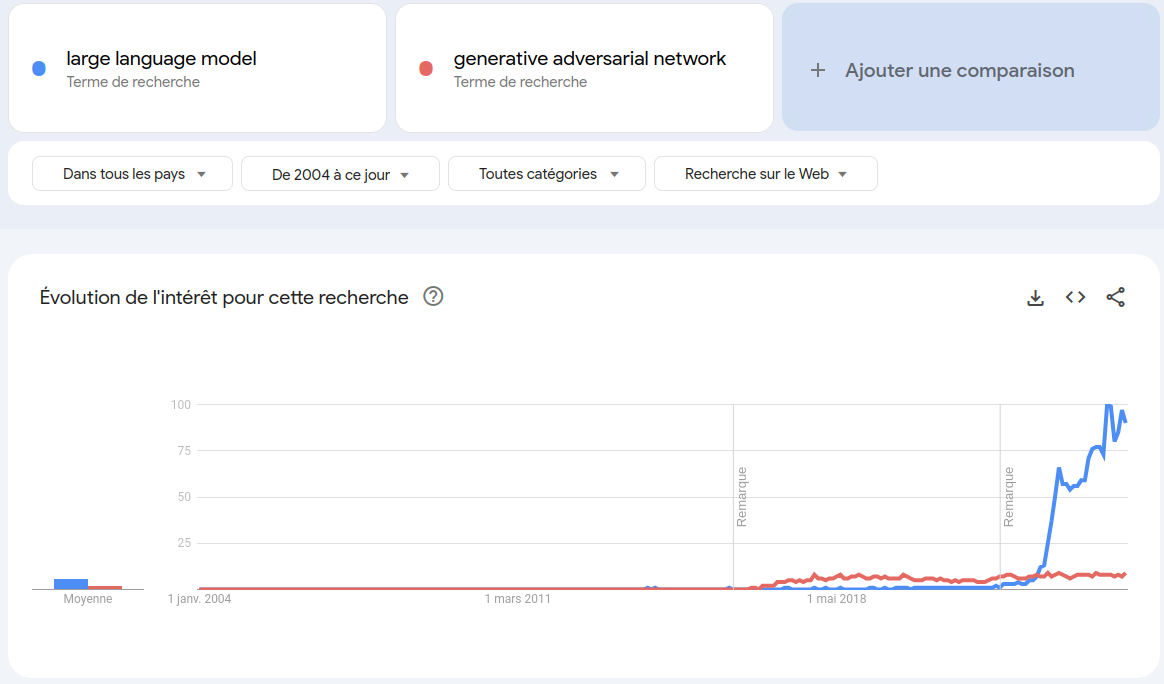
\includegraphics[width=\linewidth]{f/pop_llm_gan.png}}%
\only<2>{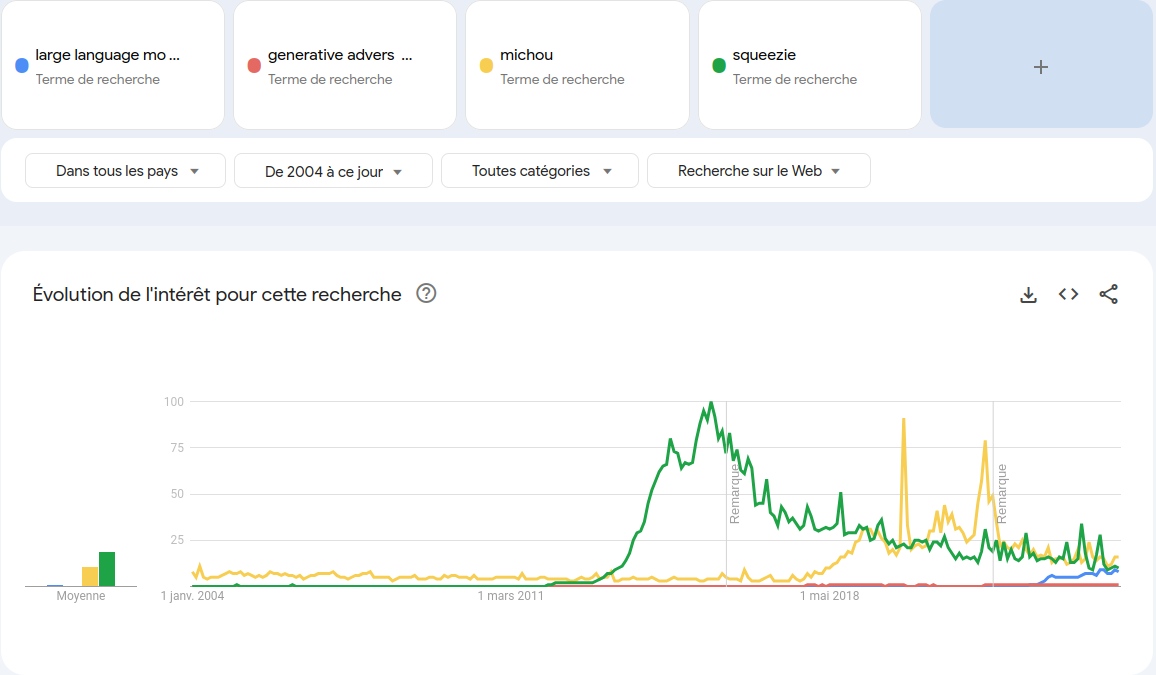
\includegraphics[width=\linewidth]{f/pop_llm_gan2.png}}%
\only<3>{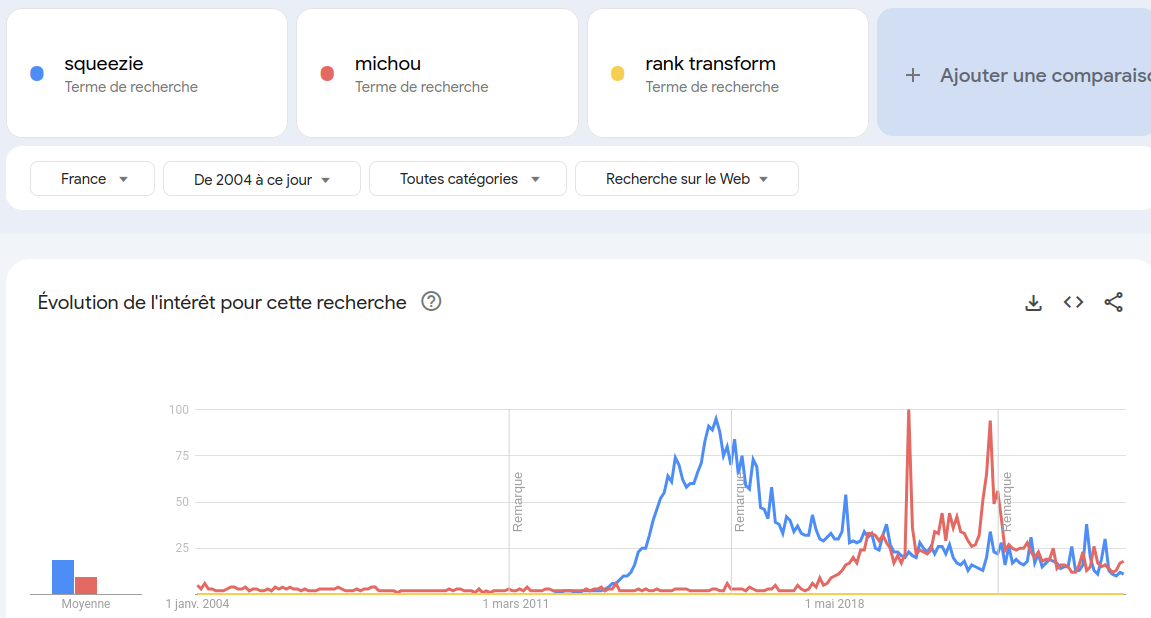
\includegraphics[width=\linewidth]{f/pop_rt.png}}%

Source: {\color{blue}http://trends.google.fr/}
%GOOGLE TRENDS\\
%=============
%
%	(the joke about popularity being the opposite of originality, with some
%	related graphs of google trends)
\end{frame}


\begin{frame}
OUTLINE\\
=======

\vfill

1. Rank Transform\\
$\ \quad${\color{gray}($\approx$ 5min)}

2. Kernel Rank Transform\\
$\ \quad${\color{gray}($\approx$ 15min)}

\vfill

\end{frame}


\begin{frame}[plain,noframenumbering]%

\vfill
\begin{center}
\Huge
--1--\\Rank Transform
\end{center}
\vfill
\small
\centering
{A classical tool in statistics and image processing}
\end{frame}


% 4. rank transform in statistics
\begin{frame}
THE RANK TRANSFORM IN STATISTICS\\
================================

	\begin{tabular}{ll}
		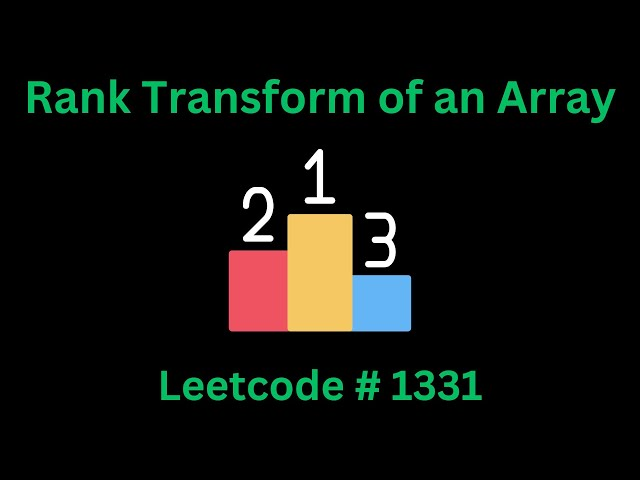
\includegraphics[height=0.3\textheight]{i/indian1.jpg}&
		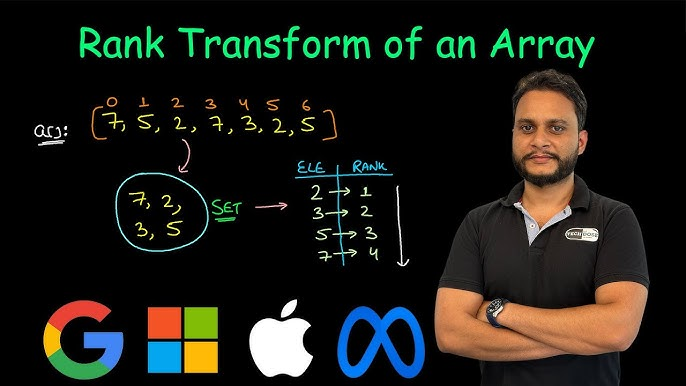
\includegraphics[height=0.3\textheight]{i/indian2.jpg}\\
	\end{tabular}\\
	$ $ Source: {\color{blue}http://www.youtube.com}


	\vfill
	\bigskip
	\vfill

	\pause
	\color{gray}\small

	[0] D.~Quade\\
	{\bf Rank analysis of covariance}\\
	{Journal of the American Statistical Association}, 1967


	[1]  W.~J.~Conover, R.~L.~Iman\\
	{\bf Analysis of covariance using the rank transformation}\\
	{Biometrics}, 1982



\end{frame}

% 5. rank transform in image processing (definitions)
\begin{frame}
THE RANK TRANSFORM IN IMAGE PROCESSING\\
======================================

{\scriptsize\color{gray}
	[2] R.~Zabih, J.~Woodfill\\
	{\bf Non-parametric Local Transforms for Computing Visual Correspondence}\\
	{ECCV, 1994}\\
}
\vspace{-0.5em}
\begin{center}
	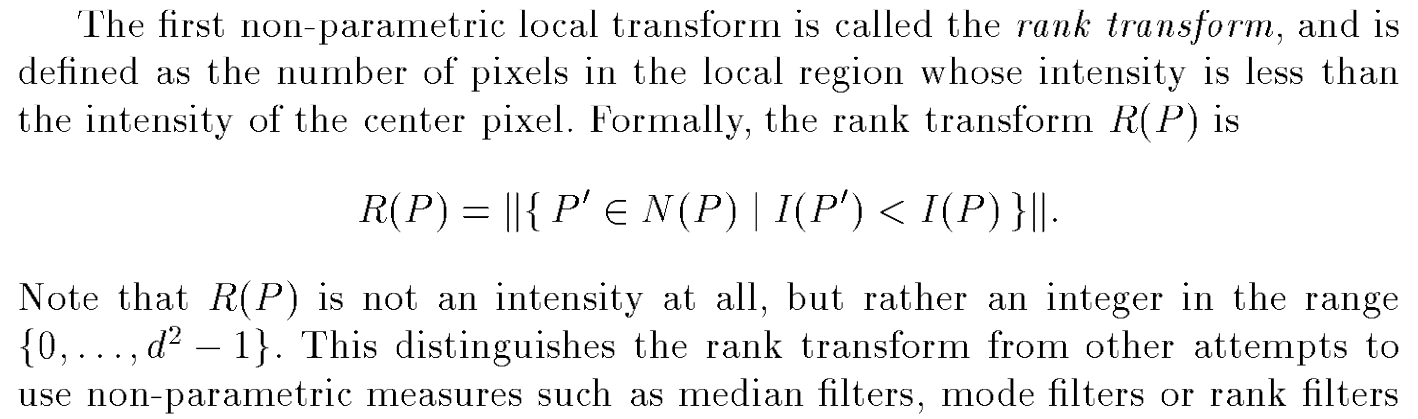
\includegraphics[width=0.7\textwidth]{i/rtdef87.png}
\end{center}

\vfill
\pause

{\scriptsize\color{gray}
	[3] O.~Demetz, D.~Hafner, J.~Weickert\\
	{\bf The Complete Rank Transform}\\
	{BMVC}, 2013\\
}
\vspace{-0.5em}
\begin{center}
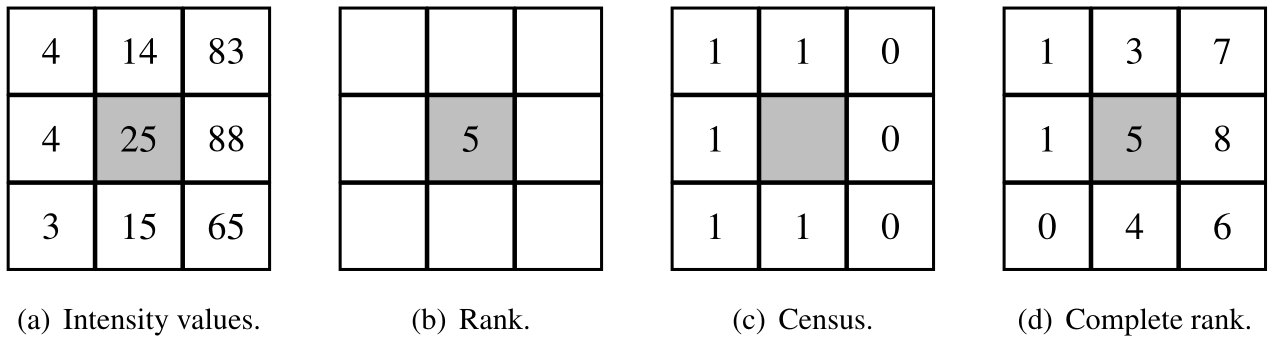
\includegraphics[width=0.7\textwidth]{i/rtfig13.png}
\end{center}



\end{frame}

% (no)6. visualization of the rank transform of various images and window sizes
\begin{frame}
PROPERTIES OF THE RANK TRANSFORM\\
================================

{\bf 1. Contrast-invariance.}
	For increasing~$g:\textbf{R}\to\textbf{R}$:
	\[
		\textsc{RT}_d(u) = \textsc{RT}_d(g\circ u)
	\]

	{\bf 2. Histogram equalization.}
	\[\displaystyle\lim_{d\to\infty}\textsc{RT}_d(u)=\varphi\circ u\]
	where~$\varphi$ is the cumulative distribution function of~$u$.

	{\bf 3. Visual effect of the parameter }$d$

\end{frame}

% (no)
% 7. first observation: small window=curvature, large window=histogram equaliz.
\begin{frame}
FIRST MYSTERY: LINK WITH CURVATURE?
===================================

%MAKE all: o/fujik.png  o/fujikd.png
%MAKE all: o/fujir5.png o/fujir5d.png
%MAKE o/fujik.png: i/fuji.tif; plambda $^ 'x,g dup vnorm /'|plambda 'x,d -1 *'|palette -1.3 1.3 nice -l OVERLAY - $@
%MAKE o/fujir5.png: i/fuji.tif; ./krt actualsquare5 $^ |palette 0 1 nice -l OVERLAY - $@
%MAKE o/fujikd.png: o/fujik.png; plambda TRANS[x=311,y=194,w=200,h=150]:$^ x|ntiply 4 - $@
%MAKE o/fujir5d.png: o/fujir5.png; plambda TRANS[x=311,y=194,w=200,h=150]:$^ x|ntiply 4 - $@

\begin{tabular}{cc}
	\small$\mathrm{div}\left(\frac{\nabla u}{\left\|\nabla u\right\|}\right)$ &
	$\textsc{RT}_5(u)$ \\
	\includegraphics[height=0.38\textheight]{o/fujik.png}&
	\includegraphics[height=0.38\textheight]{o/fujir5.png}\\
	\includegraphics[height=0.38\textheight]{o/fujikd.png}&
	\includegraphics[height=0.38\textheight]{o/fujir5d.png}\\
\end{tabular}


\end{frame}

% 8. integral formulation of the classical rank transform
\begin{frame}
INTEGRAL FORMULATION OF THE RANK TRANSFORM\\
==========================================
\end{frame}

% 9. generalization: the KRT
\begin{frame}
GENERALIZATION OF THE INTEGRAL FORMULATION\\
==========================================
\end{frame}


\begin{frame}[plain,noframenumbering]%

\vfill
\begin{center}
\Huge
--2--\\Kernel Rank Transform
\end{center}
\vfill
\small
\centering
{the subject of our study}
\end{frame}

% 10. formal definition, common gaussian/heaviside cases, generalizes RT
% 11. first formal properties (extreme cases of the parameters)
% 12. visual exploration of the parameters
% 13. first implementation (c code)
% 14. structural properties
% 15. theorem about contrast invariance being a non-differentiable property
% 16. limit for a large kernel
% 17. limit for a vanishingly small kernel, link with curvature (thm)
% 18. ref. alvarez guichard lions evans
% 19. implementation as a convolution in 3D

% 20. particular cases of the KRT, common operators, applications
%   20.1. retinex
%   20.2. dsm/depth image exploration
%   20.3. bilateral filtering
%   20.4. normalizatoin prior to matching (examples w/ cross-correlation scores)
% 21. comparison with other ``whitening'' transforms
%   21.1. laplacian
%   21.2. gradient direction image
%   21.3. integrated gradient direction image
%   21.4. phase image
%   21.5. x-blurred(x)
%   21.6. x-denoised(x)
% 22. summary of particular cases as a 2d table
% 23. choice of implementation depending on parameters
% 24. comparison with perceptron layers / implementation in npu ?

% 25. colophon: source code of the article and the presentation





% 10. formal definition, common gaussian/heaviside cases, generalizes RT
\begin{frame}
DEFINITION OF THE KRT\\
=====================
\end{frame}

% 11. first formal properties (extreme cases of the parameters)
\begin{frame}
FORMAL PROPERTIES (I)\\
=====================
\end{frame}

\begin{frame}
FORMAL PROPERTIES (II)\\
======================
\end{frame}

% 12. visual exploration of the parameters
\begin{frame}
EXPLORATION OF THE PARAMETERS\\
=============================
\end{frame}

% 13. first implementation (c code)
\begin{frame}
IMPLEMENTATION\\
==============

	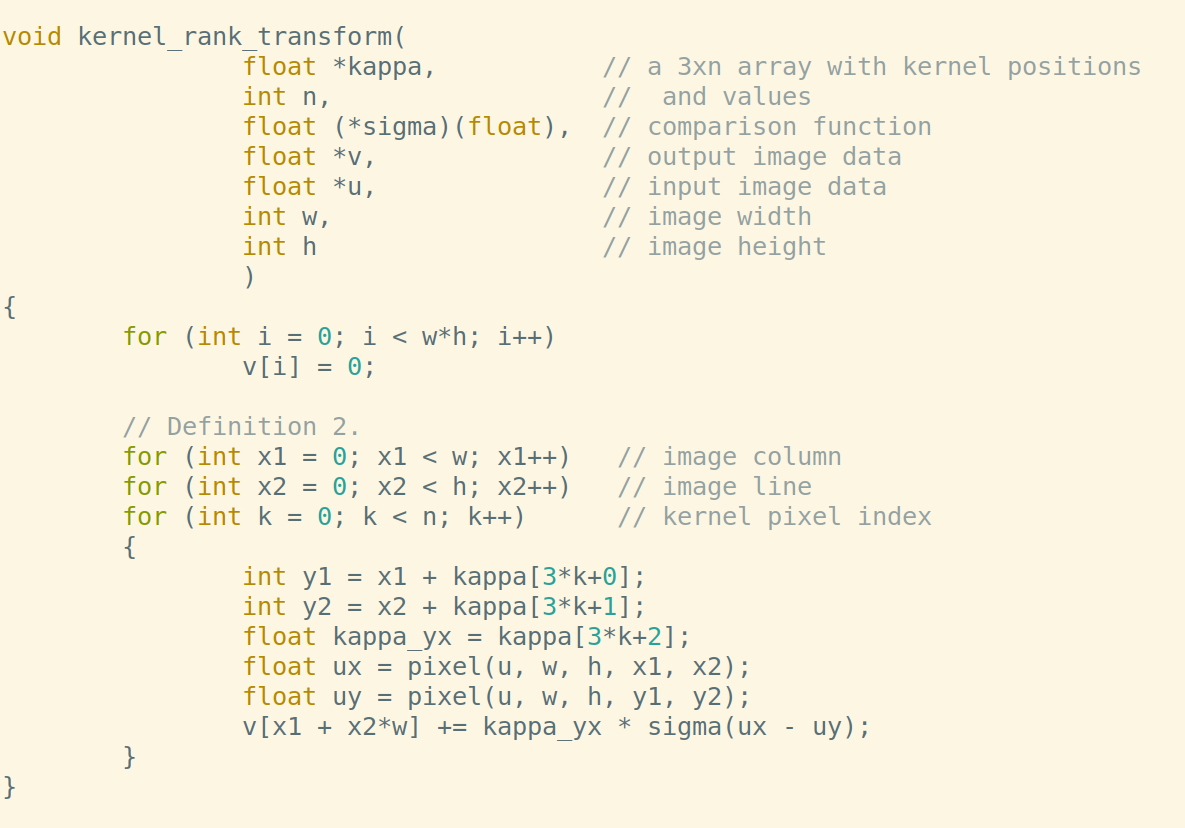
\includegraphics[width=\textwidth]{i/krtcode.png}

\end{frame}

% 14. structural properties
\begin{frame}
STRUCTURAL PROPERTIES\\
=====================
\end{frame}

% 15. theorem about contrast invariance being a non-differentiable property
\begin{frame}
CONTRAST INVARIANCE\\
===================
\end{frame}

% 16. limit for a large kernel
\begin{frame}
LIMIT FOR LARGE KERNELS\\
=======================
\end{frame}

% 17. limit for a vanishingly small kernel, link with curvature (thm)
\begin{frame}
LIMIT FOR SMALL KERNELS\\
=======================

	(maybe separate the cases into two or three slides)
\end{frame}

% 18. ref. alvarez guichard lions evans
\begin{frame}
	(ref. alvarez guichard lions evans)
\end{frame}

% 19. implementation as a convolution in 3D
\begin{frame}
INTERPRETATION IN 3D\\
====================
\end{frame}


% 20. particular cases of the KRT, common operators, applications
\begin{frame}
PARTICULAR CASES OF THE KRT\\
===========================
\end{frame}

%   20.1. retinex
\begin{frame}
	retinex\\
=============
\end{frame}

%   20.2. dsm/depth image exploration
\begin{frame}
	dsm/depth image exploration\\
=============
\end{frame}

%   20.3. bilateral filtering
\begin{frame}
	bilateral filtering\\
=============
\end{frame}

%   20.4. normalizatoin prior to matching (examples w/ cross-correlation scores)
\begin{frame}
	normalization prior to matching\\
=============
\end{frame}

% 21. comparison with other ``whitening'' transforms
\begin{frame}
COMPARISON WITH OTHER ``WHITENING'' TRANSFORMS\\
==============================================
\end{frame}

%%   21.1. laplacian
%\begin{frame}
%=============
%\end{frame}
%
%%   21.2. gradient direction image
%\begin{frame}
%=============
%\end{frame}
%
%%   21.3. integrated gradient direction image
%\begin{frame}
%=============
%\end{frame}
%
%%   21.4. phase image
%\begin{frame}
%=============
%\end{frame}
%
%%   21.5. x-blurred(x)
%\begin{frame}
%=============
%\end{frame}
%
%%   21.6. x-denoised(x)
%\begin{frame}
%=============
%\end{frame}

% 22. summary of particular cases as a 2d table
\begin{frame}
PARTICULAR CASES OF THE KRT\\
===========================
\end{frame}

% 23. choice of implementation depending on parameters
\begin{frame}
CHOICE OF IMPLEMENTATION DEPENDING ON THE PARAMETERS\\
====================================================
\end{frame}

% 24. comparison with perceptron layers / implementation in npu ?
\begin{frame}
COMPARISON WITH A PERCEPTRON LAYER\\
==================================
\end{frame}


% 25. colophon: source code of the article and the presentation
\begin{frame}
COLOPHON\\
========
\end{frame}






\end{document}


% vim:sw=2 ts=2 :
